% Seção 1: Introdução às Redes 5G

\section{Introdução às Redes 5G}
\begin{frame}
    \frametitle{O que é o 5G?}
    \begin{itemize}
        \item Quinta geração de redes móveis.
        \item Promete velocidades ultrarrápidas, latência ultrabaixa e conectividade massiva.
        \item Suporte a novas aplicações, como IoT, realidade aumentada/virtual, veículos autônomos.
    \end{itemize}
\end{frame}

\begin{frame}
    \frametitle{Arquitetura do 5G}
    \begin{itemize}
        \item \textbf{Rede de Acesso por Rádio (RAN)}: Nova radiofrequência e técnicas avançadas de transmissão.
        \item \textbf{Rede Central (Core)}: Baseada em software, mais flexível e ágil.
        \item \textbf{Suporte Multisserviço}: \textit{Network slicing} para diferentes tipos de serviços.
    \end{itemize}
    \begin{figure}
        \centering
        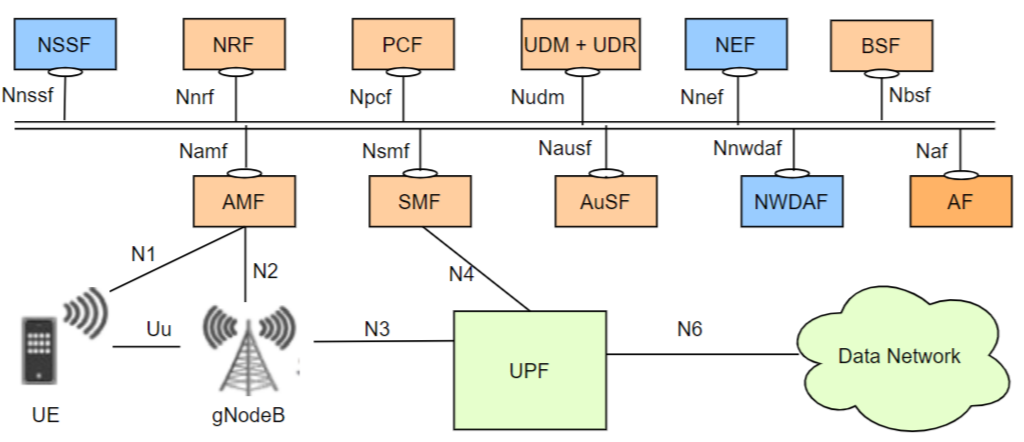
\includegraphics[width=0.7\textwidth]{figs/ArquiteturaGeral5G}
        \caption{Arquitetura Geral do 5G\footcite{5G_architecture}}
    \end{figure}
    \vspace{0.4cm}
\end{frame}

\begin{frame}
    \frametitle{Características Técnicas do 5G}
    \begin{itemize}
        \item \textbf{Velocidade}: Até 20 Gbps.
        \item \textbf{Latência}: Menos de 1 ms.
        \item \textbf{Conectividade Massiva}: Suporte para até 1 milhão de dispositivos por km².
        \item \textbf{Eficiência Espectral}: Utilização otimizada do espectro.
    \end{itemize}
    \begin{figure}
        \centering
        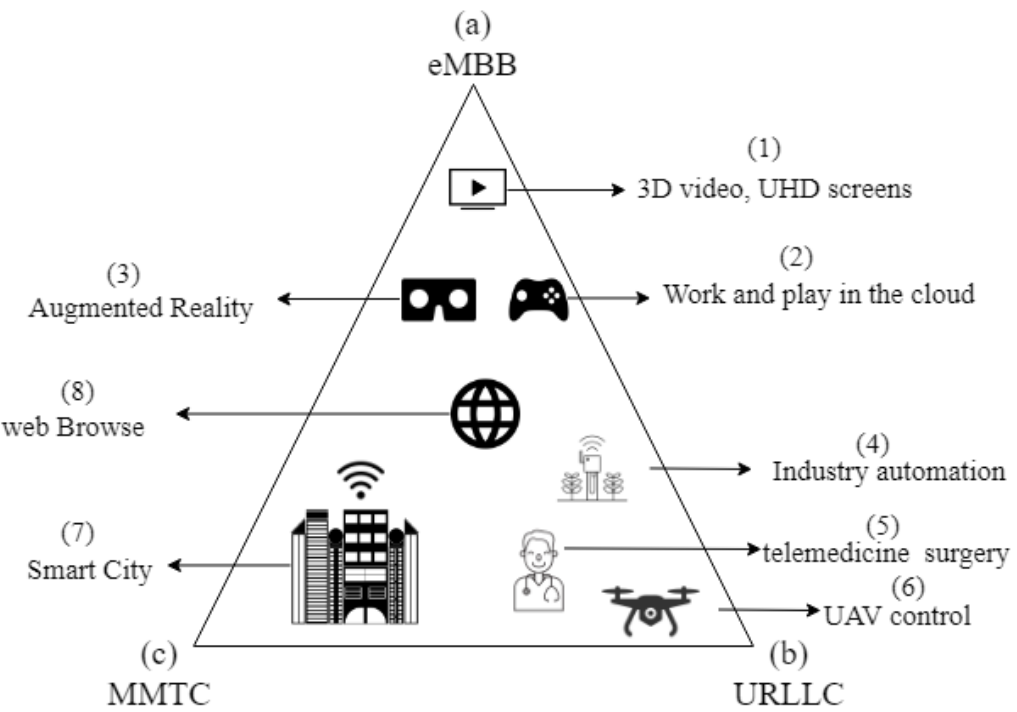
\includegraphics[width=0.5\linewidth]{figs/5G_verticais.png}
        \caption{Requisitos para diferentes tipos de aplicações\footcite{5G_verticais}}
    \end{figure}
\end{frame}
